%! Author = dmitriy
%! Date = 9/15/23

% Preamble
\documentclass[14pt]{extreport}
\usepackage{gost}
\usepackage{ragged2e}
%\usepackage{blindtext}
\justifying
\renewcommand{\thefigure}{\arabic{figure}}
\renewcommand{\thetable}{\arabic{table}}

\begin{document}
    \pagestyle{empty}
    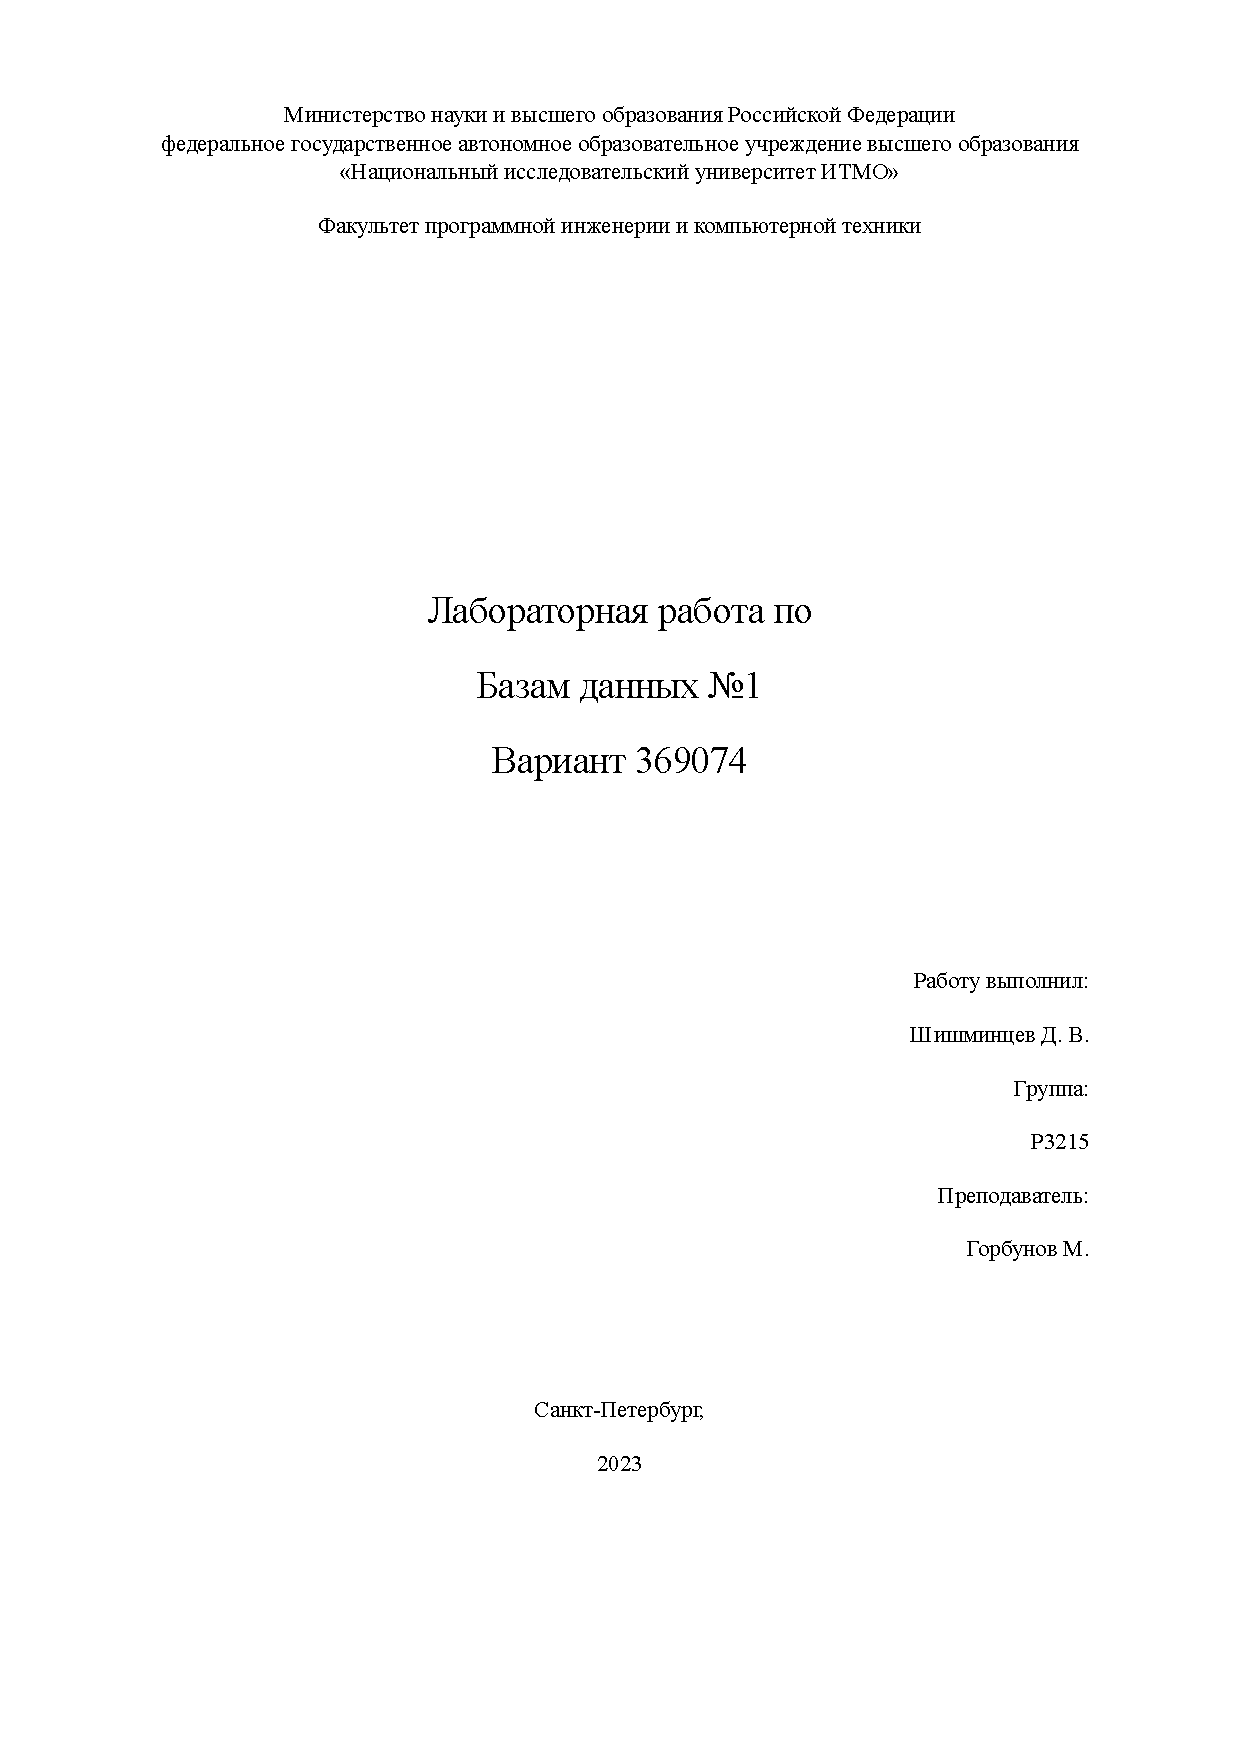
\includepdf[pages=-,pagecommand={}]{title.pdf}
    \pagestyle{plain}
    \tableofcontents

    \intro В рамках данного запроса мы будем проводить различные операции с базой данных, используя язык SQL. Запросы направлены на извлечение нужной информации из нескольких таблиц и применение различных условий, фильтров, а также соединений для получения точных данных в соответствии с заданными критериями.

    \chapter{Предметная область}
    \section{Текст задания}\\
            Сделать запрос для получения атрибутов из указанных таблиц, применив фильтры по указанным условиям:\\
            Н\_ТИПЫ\_ВЕДОМОСТЕЙ, Н\_ВЕДОМОСТИ.\\
            Вывести атрибуты: Н\_ТИПЫ\_ВЕДОМОСТЕЙ.НАИМЕНОВАНИЕ, Н\_ВЕДОМОСТИ.ИД.\\
            Фильтры (AND):\\
            a) Н\_ТИПЫ\_ВЕДОМОСТЕЙ.НАИМЕНОВАНИЕ = Ведомость.\\
            b) Н\_ВЕДОМОСТИ.ЧЛВК\_ИД = 117219.\\
            Вид соединения: INNER JOIN.\\
            Сделать запрос для получения атрибутов из указанных таблиц, применив фильтры по указанным условиям:\\
            Таблицы: Н\_ЛЮДИ, Н\_ВЕДОМОСТИ, Н\_СЕССИЯ.\\
            Вывести атрибуты: Н\_ЛЮДИ.ФАМИЛИЯ, Н\_ВЕДОМОСТИ.ЧЛВК\_ИД, Н\_СЕССИЯ.ЧЛВК\_ИД.\\
            Фильтры (AND):\\
            a) Н\_ЛЮДИ.ИД = 100865.\\
            b) Н\_ВЕДОМОСТИ.ИД < 39921.\\
            c) Н\_СЕССИЯ.ЧЛВК\_ИД > 151200.\\
            Вид соединения: INNER JOIN.\\
            Вывести число имен без учета повторений.\\
            При составлении запроса нельзя использовать DISTINCT.\\
            Найти группы, в которых в 2011 году было ровно 10 обучающихся студентов на кафедре вычислительной техники.\\
            Для реализации использовать соединение таблиц.\\
            Выведите таблицу со средними оценками студентов группы 4100 (Номер, ФИО, Ср\_оценка), у которых средняя оценка не больше минимальной оценк(е|и) в группе 1100.\\
            Получить список студентов, зачисленных после первого сентября 2012 года на первый курс очной или заочной формы обучения. В результат включить: \\
            номер группы;\\
            номер, фамилию, имя и отчество студента;\\
            номер и состояние пункта приказа;\\
            Для реализации использовать подзапрос с EXISTS. \\
            Вывести список студентов, имеющих одинаковые отчества, но не совпадающие даты рождения. \\

\section{1 Задание}
    \section{Запросы}
        \begin{verbatim}
-- 1 Запрос:
SELECT Н_ТИПЫ_ВЕДОМОСТЕЙ.НАИМЕНОВАНИЕ,
       Н_ВЕДОМОСТИ.ИД
FROM Н_ТИПЫ_ВЕДОМОСТЕЙ
INNER JOIN Н_ВЕДОМОСТИ ON Н_ТИПЫ_ВЕДОМОСТЕЙ.ИД = Н_ВЕДОМОСТИ.ИД
WHERE Н_ТИПЫ_ВЕДОМОСТЕЙ.НАИМЕНОВАНИЕ = 'Ведомость'
  AND Н_ВЕДОМОСТИ.ЧЛВК_ИД = 117219;

-- 2 Запрос:
SELECT Н_ЛЮДИ.ФАМИЛИЯ,
       Н_ВЕДОМОСТИ.ЧЛВК_ИД,
       Н_СЕССИЯ.ЧЛВК_ИД
FROM Н_ЛЮДИ
INNER JOIN Н_ВЕДОМОСТИ ON Н_ЛЮДИ.ИД = Н_ВЕДОМОСТИ.ЧЛВК_ИД
INNER JOIN Н_СЕССИЯ ON Н_ЛЮДИ.ИД = Н_СЕССИЯ.ЧЛВК_ИД
WHERE Н_ЛЮДИ.ИД = 100865
  AND Н_ВЕДОМОСТИ.ИД < 39921
  AND Н_СЕССИЯ.ЧЛВК_ИД > 151200;

-- 3 Запрос:
SELECT COUNT(*)
FROM
  (SELECT ИМЯ
   FROM Н_ЛЮДИ
   GROUP BY ИМЯ) AS UNIQUE_NANES

-- 4 Запрос:
SELECT count("Н_УЧЕНИКИ")
FROM "Н_ОТДЕЛЫ"
JOIN "Н_ПЛАНЫ" ON "Н_ПЛАНЫ"."ОТД_ИД" = "Н_ОТДЕЛЫ"."ИД"
JOIN "Н_ГРУППЫ_ПЛАНОВ" ON "Н_ГРУППЫ_ПЛАНОВ"."ПЛАН_ИД" = "Н_ПЛАНЫ"."ИД"
JOIN "Н_УЧЕНИКИ" ON "Н_УЧЕНИКИ"."ГРУППА" = "Н_ГРУППЫ_ПЛАНОВ"."ГРУППА"
WHERE "Н_ОТДЕЛЫ"."КОРОТКОЕ_ИМЯ" = 'ВТ'
  AND "Н_ПЛАНЫ"."УЧЕБНЫЙ_ГОД" = '2011'
GROUP BY "Н_ГРУППЫ_ПЛАНОВ"."ГРУППА"
HAVING count("Н_УЧЕНИКИ") = 10;

-- 5 Запрос:
SELECT "ЧЛВК_ИД" AS "НОМЕР",
       CONCAT("ФАМИЛИЯ", ' ', "ИМЯ", ' ', "ОТЧЕСТВО") AS "ФИО",
       "СР_ОЦЕНКА"
FROM
    (SELECT "ЧЛВК_ИД",
            AVG(ОЦЕНКА::integer) AS "СР_ОЦЕНКА"
     FROM
         (SELECT "Н_ВЕДОМОСТИ"."ОЦЕНКА",
                 "Н_ВЕДОМОСТИ"."ЧЛВК_ИД",
                 "Н_УЧЕНИКИ"."ГРУППА"
          FROM "Н_ВЕДОМОСТИ"
                   LEFT JOIN "Н_УЧЕНИКИ" ON
                      "Н_ВЕДОМОСТИ"."ЧЛВК_ИД" = "Н_УЧЕНИКИ"."ЧЛВК_ИД"
          WHERE "ОЦЕНКА" ~ '^[0-9]+$'
            AND "ГРУППА"::integer = 4100 ) AS STUDENTS
     GROUP BY "ЧЛВК_ИД") AS AVERAGE_MARKS
        LEFT JOIN "Н_ЛЮДИ" ON AVERAGE_MARKS."ЧЛВК_ИД" = "Н_ЛЮДИ"."ИД"
WHERE "СР_ОЦЕНКА">
      (SELECT MIN("ОЦЕНКА")
       FROM
           (SELECT "Н_ВЕДОМОСТИ"."ОЦЕНКА",
                   "Н_ВЕДОМОСТИ"."ЧЛВК_ИД",
                   "Н_УЧЕНИКИ"."ГРУППА"
            FROM "Н_ВЕДОМОСТИ"
                     LEFT JOIN "Н_УЧЕНИКИ" ON
                        "Н_ВЕДОМОСТИ"."ЧЛВК_ИД" = "Н_УЧЕНИКИ"."ЧЛВК_ИД"
            WHERE "ОЦЕНКА" ~ '^[0-9]+$' ) AS S1
       WHERE "ГРУППА"::integer = 1100)::integer

-- 6 запрос:
SELECT "Н_УЧЕНИКИ"."ГРУППА",
       "Н_УЧЕНИКИ"."ИД",
       "Н_ЛЮДИ"."ФАМИЛИЯ",
       "Н_ЛЮДИ"."ИМЯ",
       "Н_ЛЮДИ"."ОТЧЕСТВО",
       "Н_УЧЕНИКИ"."П_ПРКОК_ИД"
FROM "Н_ЛЮДИ"
JOIN "Н_УЧЕНИКИ" ON "Н_ЛЮДИ"."ИД" = "Н_УЧЕНИКИ"."ЧЛВК_ИД"
WHERE "Н_УЧЕНИКИ"."НАЧАЛО" > '2012-09-01'::timestamp
  AND EXISTS
    (SELECT 1
     FROM "Н_ПЛАНЫ"
     JOIN "Н_ФОРМЫ_ОБУЧЕНИЯ" ON "Н_ПЛАНЫ"."ФО_ИД" = "Н_ФОРМЫ_ОБУЧЕНИЯ"."ИД"
     WHERE "Н_ПЛАНЫ"."КУРС" = 1
       AND ("Н_ФОРМЫ_ОБУЧЕНИЯ"."НАИМЕНОВАНИЕ" = 'Заочная'
            OR "Н_ФОРМЫ_ОБУЧЕНИЯ"."НАИМЕНОВАНИЕ" = 'Очная')
       AND "Н_УЧЕНИКИ"."ПЛАН_ИД" = "Н_ПЛАНЫ"."ИД" );


-- 7 запрос:
SELECT CONCAT(s1."ФАМИЛИЯ", ' ', s1."ИМЯ", ' ', s1."ОТЧЕСТВО") AS ФИО,
       s1."ДАТА_РОЖДЕНИЯ",
       CONCAT(s2."ФАМИЛИЯ", ' ', s2."ИМЯ", ' ', s2."ОТЧЕСТВО") AS ФИО,
       s2."ДАТА_РОЖДЕНИЯ"
FROM "Н_ЛЮДИ" s1
JOIN "Н_ЛЮДИ" s2 ON s1."ОТЧЕСТВО" = s2."ОТЧЕСТВО"
WHERE s1."ДАТА_РОЖДЕНИЯ" = s2."ДАТА_РОЖДЕНИЯ"
  AND s1."ИД" <> s2."ИД"
  AND s1."ОТЧЕСТВО" <> '.'
  AND s2."ОТЧЕСТВО" <> '.'
  SELECT *
  FROM "Н_ЛЮДИ"
        \end{verbatim}
    \conclusions В результате выполнения данных SQL-запросов мы получаем разнообразную информацию из базы данных в соответствии с заданными условиями, используя различные методы фильтрации, соединения и агрегации данных. SQL позволяет эффективно извлекать нужные данные и проводить различные операции для анализа информации в базе данных.
\end{document}